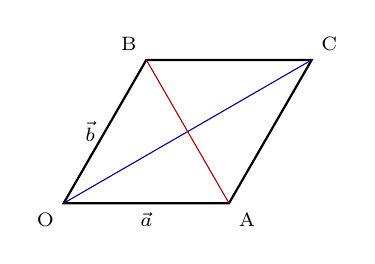
\begin{tikzpicture}[scale=0.7]
\draw[thick] (0.000,0.000)--(3.000,0.000)--(4.500,2.600)--(1.500,2.600)--cycle;\draw[blue!60!black] (0.000,0.000)--(4.500,2.600);\draw[red!70!black] (3.000,0.000)--(1.500,2.600);\node[below left] at (0.000,0.000){\scriptsize O};\node[below right] at (3.000,0.000){\scriptsize A};\node[above right] at (4.500,2.600){\scriptsize C};\node[above left] at (1.500,2.600){\scriptsize B};\node[below] at (1.500,0.000){\scriptsize $\vec a$};\node[left] at (0.750,1.300){\scriptsize $\vec b$};
\end{tikzpicture}